\subsection{Hardware test bed}
We conducted all benchmarks on a single CPU socket from Intel's \IVB and  \SKX families, respectively, since these  represent the oldest and the latest Intel architectures in active use within the scientific community at the time of writing:
\begin{itemize}
\item The \Intel \IVB architecture belongs to the class of ``classic'' designs with three inclusive cache levels. While the L1 and L2 caches are private to each core, the L3 cache is shared but scalable in terms of bandwidth. The processor supports the AVX instruction set extension, which is capable of 256-bit wide \SIMD execution.
\item Contrary to its predecessors, the \Intel \SKX architecture has a shared but noninclusive victim L3 cache and much larger private L2 caches. The model we use in this work supports AVX-512, which features 512-bit wide \SIMD execution.
%  \begin{comment}
%  \item {\GW \AMD \EPY is based on AMD's Zen microarchitecture. The basic building block of the architecture consists of Core Complex (CCX) consisting of three cores (can extend upto four on high end models) each having it's own private L1 and L2 cache. The L3 cache is shared between a core complex and is non-inclusive victim cache. A single socket of \EPY consists of eight such CCX.}
%  \end{comment}
 
\end{itemize}
Architectural details along with the attainable memory bandwidths are given in \Cref{tab:test_bed}. 
All the measurements were done with \CPU clock speeds fixed at the indicated base frequencies. Note that for the \SKX architecture the clock frequency is scaled down internally to 2.2 \GHZ when using multicore support and the AVX-512 instruction set; however, this is of minor importance for the algorithms discussed here.
\begin{comment}
\begin{table}[tbp]
\footnotesize
\caption{Compute node configurations. The last two columns present attainable bandwidth numbers ($b_S$) on a single socket, depending on the access pattern (copy vs. load only)}\label{tab:test_bed}
\begin{center}
%	\setlength{\tabcolsep}{3em}
	\begin{tabular}{|l| c  c c |}
		\toprule
		{Model name} & {Xeon\textsuperscript{\textregistered} E5-2660} & {Xeon\textsuperscript{\textregistered} Gold 6148} & { Epyc 7451 } \\
		\midrule
		{Microarchitecture} & {Ivy Bridge} & {Skylake} & {Zen} \\
		\midrule
		{Base clock frequency} & {2.2 GHz} & {2.4 GHz} & {2.3 GHz}\\
		{Physical Cores per socket} & {10} & {20} & {24}\\
		{L1d Cache} & {10 $\times$ 32 \KB} & {20 $\times$ 32 \KB} & {24 $\times$  32 \KB}\\
		{L2 Cache} & {10 $\times$ 256 \KB} & {20 $\times$ 1 \MB} & {24 $\times$ 512 \MB }\\
		{L3 Cache} & {25 \MB} & {27.5 \MB} & {8 $\times$ 8 \MB}\\
		{L3 type} & {inclusive} & {non-inclusive} & {non-inclusive}\\
		{Main Memory} & {32 GB} & {45 GB} & {4 $\times$ 16 GB}\\
		{Bandwidth per socket - load only} & {47 GB/s} & {115 GB/s} & {130 GB/s }\\ %TODO
		{Bandwidth per socket - copy} & {40 GB/s} & {104 GB/s} & {114 GB/s }\\
		\bottomrule
	\end{tabular}
\end{center}
\end{table} 
\end{comment}

\begin{table}[t]
	\centering
%	\footnotesize
	\caption{Technical details (per socket) of the Intel CPUs used for the benchmarks.\label{tab:test_bed}}
	\begin{center}
		%	\setlength{\tabcolsep}{3em}
		\begin{tabular}{l|cc}
			{Model name} & {Xeon\textsuperscript{\textregistered} E5-2660} & {Xeon\textsuperscript{\textregistered} Gold 6148} \\\midrule
			{Microarchitecture} & {\IVB} & {\SKX} \\\midrule
			{Base clock frequency} & {2.2 GHz} & {2.4 GHz}\\
			{Uncore clock frequency} & {2.2 GHz} & {2.4 GHz}\\
			{Physical cores per socket} & {10} & {20} \\
			{L1D cache} & {10 $\times$ 32 \KiB} & {20 $\times$ 32 \KiB}\\
			{L2 cache} & {10 $\times$ 256 \KiB} & {20 $\times$ 1 \MiB} \\
			{L3 cache} & {25 \MiB} & {27.5 \MiB}\\
			{L3 type} & {inclusive} & {noninclusive, victim}\\
			{Main memory} & {32 \GiB} & {48 \GiB}\\
			{Bandwidth per socket, load-only} & {47 \GBS} & {115 \GBS}\\ %TODO
			{Bandwidth per socket, copy} & {40 \GBS} & {104 \GBS}\\
		\end{tabular}
	\end{center}
\end{table} 
As the attainable main memory bandwidth is the input parameter to the \roofline model used later, we have carefully measured this value depending on the data set size for two access patterns (copy and load-only). The data presented in \Cref{fig:size_vs_bw} basically show the characteristic performance drop if data set size is too large to fit into the \acrfull{LLC}, which is an L3 cache on both architectures (cf. \Cref{tab:test_bed} for the actual sizes). 
\begin{figure}[t]
	\centering
	\subfloat[\emph{\IVB}]{\label{fig:ivy_size_vs_bw}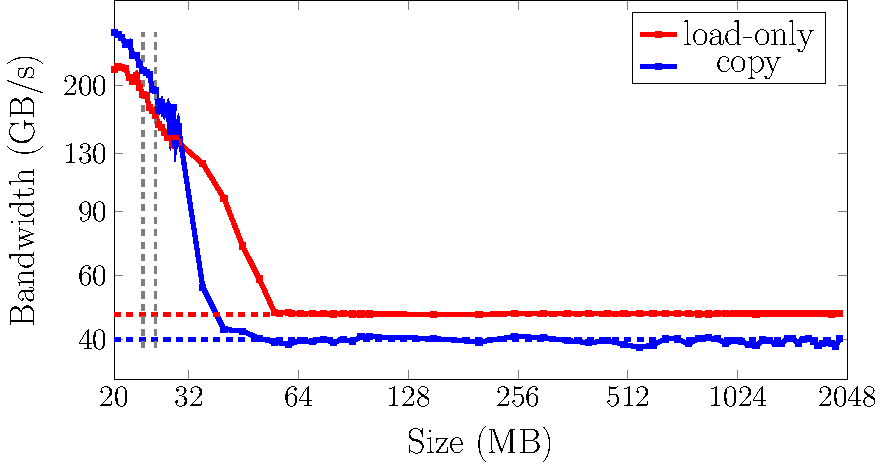
\includegraphics[width=0.5\textwidth , height=0.16\textheight]{pics/results/likwid_bench_bw/ivy}}
	\subfloat[\emph{\SKX}]{\label{fig:skx_size_vs_bw}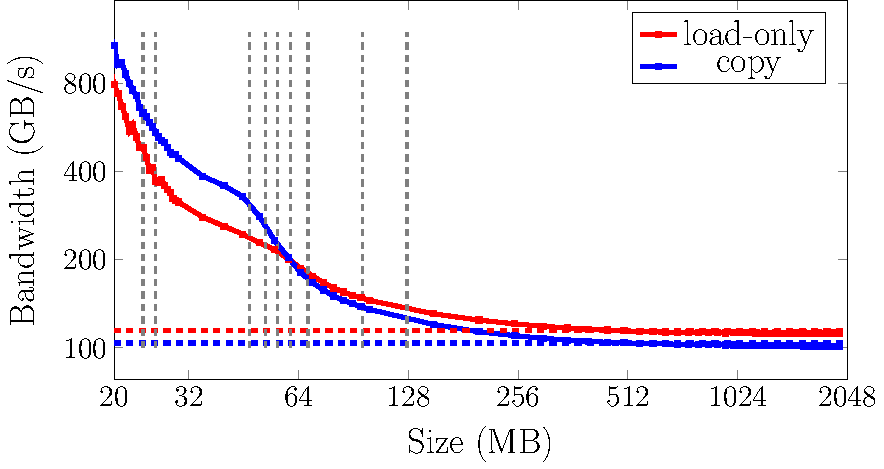
\includegraphics[width=0.5\textwidth , height=0.16\textheight]{pics/results/likwid_bench_bw/skx}}
	\caption{Attained bandwidth versus total data size for a range from 20 \MB to 2 \GB. The dotted lines show the asymptotic bandwidth given in \Cref{tab:test_bed} for the load-only and copy benchmark. The benchmarks were performed on the full socket using the \likwidBench tool. The gray vertical lines correspond to the positions of matrices that might show caching effects; see \Cref{subsec:bench_mat}. Note the logarithmic scales.}
	\label{fig:size_vs_bw}
\end{figure}
Interestingly there is no sharp drop at the exact size of the \acrshort{LLC} but a rather steady performance decrease with enhanced data access rates also for data set sizes up to twice the \acrshort{LLC} size on \IVB. For \SKX this effect is even more pronounced as the noninclusive victim L3 cache architecture only stores data which are not in the L2 cache; thus the available cache size for an application may be the aggregate sizes of the L2 and L3 caches on this architecture.  The final bandwidth for the  \roofline model is chosen as the asymptotic value depicted in \Cref{fig:size_vs_bw}. Of course caching effects are extremely sensitive to the data access pattern and thus the values presented here only provide simple upper bounds for the \acrshort{SymmSpMV} kernel with its potentially strong irregular data access. 

\subsection{External Tools and Software}
The \LIKWID \cite{LIKWID} tool suite in version 4.3.2 was used, specifically
\likwidBench for bandwidth benchmarks (see \Cref{tab:test_bed}), and
\likwidPerfctr for counting hardware events 
 and measuring derived metrics.
 \LIKWID validates the quality of it's performance metrics
  and validation data is publicly available.\footnote{\href{https://github.com/RRZE-HPC/likwid/wiki/TestAccuracy}{https://github.com/RRZE-HPC/likwid/wiki/TestAccuracy}} Overall the \LIKWID data traffic measurements can be considered as highly accurate. Only the L3 data traffic measurement on \SKX fails the quantitative validation but it still provides good qualitative results.\footnote{\href{https://github.com/RRZE-HPC/likwid/wiki/L2-L3-MEM-traffic-on-Intel-Skylake-SP-CascadeLake-SP}{https://github.com/RRZE-HPC/likwid/wiki/L2-L3-MEM-traffic-on-Intel-Skylake-SP-CascadeLake-SP}}
 
 For coloring we used the \COLPACK \cite{COLPACK} library
 and \METIS \cite{METIS} version 5.1.0 for graph partitioning
 with the \acrshort{ABMC} method. The \SPMP \cite{SpMP} library was employed for
  \acrshort{RCM} bandwidth reduction, and the \acrshort{MKL} version 19.0.2
 for some reference computations and comparisons.
%\begin{description}
%	%TODO
%	\item[\LIKWID 4.3.2] \cite{LIKWID}  \likwidPerfctr was used for counting hardware events and measuring derived metrics. The bandwidths shown in \Cref{tab:test_bed} were taken by the  \likwidBench tool.
%	\item[\COLPACK] \cite{COLPACK} was used for pre-processing matrices via \acrshort{MC}.
%	\item[\SPMP] \cite{SpMP} was used to perform \acrshort{RCM}.
%	\item[\METIS 5.1.0] \cite{METIS} was used for graph partitioning in \acrshort{ABMC}.
%	\item[\acrshort{MKL} 19.0.2] \cite{MKL} was used for performing some reference sparse matrix computations.
%\end{description}

All code was compiled with the Intel compiler in version 19.0.2 and the following compiler flags: {\tt -fno-alias -xHost -O3} for \IVB and {\tt -fno-alias -xCORE-AVX512 -O3} for \SKX.

\subsection{Benchmark Matrices}
\label{subsec:bench_mat}
Most test matrices were taken from the Suite\-Sparse Matrix Collection (formerly University of Florida Sparse Matrix Collection)~\cite{UOF} combining sets from two related papers \cite{RSB,park_ls}, which allows the reader to make a straightforward comparison of results.  We also added some matrices from the Scalable Matrix Collection (ScaMaC) library\cite{ScaMaC}, which allows for scalable generation of large matrices related to quantum physics applications. A brief description of the background of these matrices can be found in ScaMaC documentation.\footnote{\href{https://alvbit.bitbucket.io/scamac_docs/_matrices_page.html}{https://alvbit.bitbucket.io/scamac\_docs/\_matrices\_page.html}} All the matrices considered are real, although our underlying software would also support complex matrices.
%The selection of the matrices from SuiteSparse Matrix Collection is  mainly done by  Matrices from \ESSEX project are some of the matrices that are of interest in the iterative FEAST eigen value solver that internally uses Kaczmarz solver.
As mentioned before we restrict ourselves to matrices representing fully connected undirected graphs.
\Cref{table:bench_matrices} gives an overview of the most important matrix properties like \acrfull{nrows}, \acrfull{nnz}, \acrfull{NNZR}, along with the bandwidth of the matrix without ($bw$) and with ($bw_{RCM}$) \acrshort{RCM} preprocessing. 

Due to the extended cache size as seen in \Cref{fig:size_vs_bw} it
might happen that some of the matrices attain higher effective
bandwidths due to partial/full caching, especially on \SKX. The ten potential candidates
for the \SKX chip in terms of symmetric and full storage ($< 128$ \MB)
are marked with an asterisk in \Cref{table:bench_matrices}, while only
two among these (\texttt{offshore} and \texttt{parabolic\_fem}) 
satisfy the criteria for \IVB ($< 40$ \MB). The corresponding data set
size for storing the upper triangular part of these matrices have been
labeled in \Cref{fig:size_vs_bw}.

\begin{table}[t]
	\centering
%	\footnotesize
	\caption{Details of the benchmark matrices. \acrshort{nrows} is the number of matrix rows and \acrshort{nnz} is the number of nonzeros. $\acrshort{NNZR}=\acrshort{nnz}/\acrshort{nrows}$ is the average number of nonzeros per row. $bw$ and $bw_{RCM}$ refer to the matrix bandwidth without and with \acrshort{RCM} preprocessing. The letter ``C'' in the parentheses of the matrix name indicates a corner case matrix that will be discussed in detail, while the letter ``Q'' marks a matrix from quantum physics that is not part of the SuiteSparse Matrix Collection. With an asterisk (*) we have labeled all the matrices which are less than 128 \MB, which could potentially lead to some caching effects especially on the \SKX architecture. \label{tab:test_mtx}	\label{table:bench_matrices}}
	\begin{center}
		\begin{tabular}{|l|l|S[round-mode=places,round-precision=4]|S[round-mode=places,round-precision=4]|S[round-mode=places,round-precision=4]|S[round-mode=places,round-precision=4]|}
\toprule
\multirow{2}{*}{Index} & \multirow{2}{*}{Matrix name} & \multicolumn{3}{c|}{$\alpha_{SpMV}$} & {$I_{\acrshort{SpMV}}(\alpha_{SpMV})$} \\
%\midrule
\cline{3-6}
& &  {optimal} & {SKX} & {IVB} & {optimal}  \\
\midrule
{1}& {	crankseg\_1                }	& 0.004974840341951422	& 0.009900427637091272*	& 0.017876	& 0.16475420629866486	\\
{2}& {	ship\_003                  }	& 0.015054104375856307	& 0.029661678743938248*	& 0.039038	& 0.16101095659221026	\\
{3}& {	pwtk                      }	& 0.018730450092715727	& 0.03677214142565592*	& 0.038276	& 0.1596876177714501	\\
{4}& {	offshore                  }	& 0.061232390023872055	& 0.11539864519682566*	& 0.105831	& 0.14583098113326293	\\
{5}& {	F1                        }	& 0.012810282496064584	& 0.025296509558520128*	& 0.043622	& 0.16182947693011468	\\
{6}& {	inline\_1                  }	& 0.013681750417974054	& 0.013709	& 0.034046	& 0.16151058900649082	\\
{7}& {	parabolic\_fem             }	& 0.14309623622555628	& 0.25036603514337963*	& 0.224973	& 0.12494772020022805	\\
{8}& {	gsm\_106857                }	& 0.02708985058701268	& 0.052750692788036055*	& 0.094584	& 0.15675804527541276	\\
{9}& {	Fault\_639                 }	& 0.022324366119157866	& 0.045281	& 0.086085	& 0.15841480951843234	\\
{10}& {	Hubbard-12                }	& 0.07692947982285911	& 0.14286818452683273*	& 0.231786	& 0.14130255800224512	\\
{11}& {	Emilia\_923                }	& 0.022512653462004855	& 0.08265	& 0.085462	& 0.15834868547473438	\\
{12}& {	audikw\_1                  }	& 0.012152898336217176	& 0.062422	& 0.063762	& 0.16207086168751325	\\
{13}& {	bone010                   }	& 0.013768014517655372	& 0.049208	& 0.052338	& 0.16147909155409917	\\
{14}& {	dielFilterV3real          }	& 0.01234882033880347	& 0.072827	& 0.067509	& 0.16199884583462107	\\
{15}& {	thermal2                  }	& 0.14312355713563962	& 0.2504078517886007*	& 0.227709	& 0.12494174903463444	\\
{16}& {	Serena                    }	& 0.02156070528689192	& 0.100582	& 0.115621	& 0.15868356434880437	\\
{17}& {	Geo\_1438                  }	& 0.022768134283905977	& 0.089589	& 0.091725	& 0.15825905217944752	\\
{18}& {	Hook\_1498                 }	& 0.024591034497360605	& 0.103075	& 0.094818	& 0.1576224362116434	\\
{19}& {	Flan\_1565                 }	& 0.013328053114104274	& 0.054135	& 0.052516	& 0.161639862432339	\\
{20}& {	G3\_circuit                }	& 0.20695912474502637	& 0.34294305499160477*	& 0.335974	& 0.11239203379889182	\\
{21}& {	Anderson-16.5             }	& 0.14285714285714285	& 0.363368	& 0.318715	& 0.125	\\
{22}& {	FreeBosonChain-18         }	& 0.08024691655235494	& 0.27076	& 0.262774	& 0.14038128167567254	\\
{23}& {	nlpkkt120                 }	& 0.03657773850304069	& 0.160002	& 0.165642	& 0.15356057042478993	\\
{24}& {	channel-500x100x100-b050  }	& 0.05325806761196896	& 0.173504	& 0.133898	& 0.14824449726378677	\\
{25}& {	HPCG-192                  }	& 0.03742553488106633	& 0.135801	& 0.139089	& 0.15328119500901655	\\
{26}& {	FreeFermionChain-26       }	& 0.07396449704142012	& 0.387859	& 0.397282	& 0.1421362489486964	\\
{27}& {	Spin-26                   }	& 0.07142857142857142	& 0.367034	& 0.351781	& 0.14285714285714285	\\
{28}& {	Hubbard-14                }	& 0.06666796002509115	& 0.357508	& 0.359807	& 0.14423039256024434	\\
{29}& {	nlpkkt200                 }	& 0.036231752783504406	& 0.16692	& 0.172028	& 0.15367487636455557	\\
{30}& {	delaunay\_n24              }	& 0.1666668333335	& 0.406459	& 0.319197	& 0.1199999663999758	\\
{31}& {	Graphene-4096             }	& 0.0769548711240621	& 0.160392	& 0.127774	& 0.14129546073388705	\\
%#TABLE_DATA#
\bottomrule
\end{tabular}



	\end{center}
\end{table}

%\begin{table}[ht]
%	\footnotesize
%	\caption{Scamac matrices} \label{tab:test_mtx_scamac}
%	\begin{center}
%		\begin{tabular}{|l|l|S[round-mode=places,round-precision=4]|S[round-mode=places,round-precision=4]|S[round-mode=places,round-precision=4]|S[round-mode=places,round-precision=4]|}
\toprule
\multirow{2}{*}{Index} & \multirow{2}{*}{Matrix name} & \multicolumn{3}{c|}{$\alpha_{SpMV}$} & {$I_{\acrshort{SpMV}}(\alpha_{SpMV})$} \\
%\midrule
\cline{3-6}
& &  {optimal} & {SKX} & {IVB} & {optimal}  \\
\midrule
{1}& {	crankseg\_1                }	& 0.004974840341951422	& 0.009900427637091272*	& 0.017876	& 0.16475420629866486	\\
{2}& {	ship\_003                  }	& 0.015054104375856307	& 0.029661678743938248*	& 0.039038	& 0.16101095659221026	\\
{3}& {	pwtk                      }	& 0.018730450092715727	& 0.03677214142565592*	& 0.038276	& 0.1596876177714501	\\
{4}& {	offshore                  }	& 0.061232390023872055	& 0.11539864519682566*	& 0.105831	& 0.14583098113326293	\\
{5}& {	F1                        }	& 0.012810282496064584	& 0.025296509558520128*	& 0.043622	& 0.16182947693011468	\\
{6}& {	inline\_1                  }	& 0.013681750417974054	& 0.013709	& 0.034046	& 0.16151058900649082	\\
{7}& {	parabolic\_fem             }	& 0.14309623622555628	& 0.25036603514337963*	& 0.224973	& 0.12494772020022805	\\
{8}& {	gsm\_106857                }	& 0.02708985058701268	& 0.052750692788036055*	& 0.094584	& 0.15675804527541276	\\
{9}& {	Fault\_639                 }	& 0.022324366119157866	& 0.045281	& 0.086085	& 0.15841480951843234	\\
{10}& {	Hubbard-12                }	& 0.07692947982285911	& 0.14286818452683273*	& 0.231786	& 0.14130255800224512	\\
{11}& {	Emilia\_923                }	& 0.022512653462004855	& 0.08265	& 0.085462	& 0.15834868547473438	\\
{12}& {	audikw\_1                  }	& 0.012152898336217176	& 0.062422	& 0.063762	& 0.16207086168751325	\\
{13}& {	bone010                   }	& 0.013768014517655372	& 0.049208	& 0.052338	& 0.16147909155409917	\\
{14}& {	dielFilterV3real          }	& 0.01234882033880347	& 0.072827	& 0.067509	& 0.16199884583462107	\\
{15}& {	thermal2                  }	& 0.14312355713563962	& 0.2504078517886007*	& 0.227709	& 0.12494174903463444	\\
{16}& {	Serena                    }	& 0.02156070528689192	& 0.100582	& 0.115621	& 0.15868356434880437	\\
{17}& {	Geo\_1438                  }	& 0.022768134283905977	& 0.089589	& 0.091725	& 0.15825905217944752	\\
{18}& {	Hook\_1498                 }	& 0.024591034497360605	& 0.103075	& 0.094818	& 0.1576224362116434	\\
{19}& {	Flan\_1565                 }	& 0.013328053114104274	& 0.054135	& 0.052516	& 0.161639862432339	\\
{20}& {	G3\_circuit                }	& 0.20695912474502637	& 0.34294305499160477*	& 0.335974	& 0.11239203379889182	\\
{21}& {	Anderson-16.5             }	& 0.14285714285714285	& 0.363368	& 0.318715	& 0.125	\\
{22}& {	FreeBosonChain-18         }	& 0.08024691655235494	& 0.27076	& 0.262774	& 0.14038128167567254	\\
{23}& {	nlpkkt120                 }	& 0.03657773850304069	& 0.160002	& 0.165642	& 0.15356057042478993	\\
{24}& {	channel-500x100x100-b050  }	& 0.05325806761196896	& 0.173504	& 0.133898	& 0.14824449726378677	\\
{25}& {	HPCG-192                  }	& 0.03742553488106633	& 0.135801	& 0.139089	& 0.15328119500901655	\\
{26}& {	FreeFermionChain-26       }	& 0.07396449704142012	& 0.387859	& 0.397282	& 0.1421362489486964	\\
{27}& {	Spin-26                   }	& 0.07142857142857142	& 0.367034	& 0.351781	& 0.14285714285714285	\\
{28}& {	Hubbard-14                }	& 0.06666796002509115	& 0.357508	& 0.359807	& 0.14423039256024434	\\
{29}& {	nlpkkt200                 }	& 0.036231752783504406	& 0.16692	& 0.172028	& 0.15367487636455557	\\
{30}& {	delaunay\_n24              }	& 0.1666668333335	& 0.406459	& 0.319197	& 0.1199999663999758	\\
{31}& {	Graphene-4096             }	& 0.0769548711240621	& 0.160392	& 0.127774	& 0.14129546073388705	\\
%#TABLE_DATA#
\bottomrule
\end{tabular}



%	\end{center}
%\end{table}

%\begin{table}[ht]
%	\footnotesize
%	\caption{nlpkkt matrices} \label{tab:test_mtx_nlpkkt}
%	\begin{center}
%		\begin{tabular}{|l|l|S[round-mode=places,round-precision=4]|S[round-mode=places,round-precision=4]|S[round-mode=places,round-precision=4]|S[round-mode=places,round-precision=4]|}
\toprule
\multirow{2}{*}{Index} & \multirow{2}{*}{Matrix name} & \multicolumn{3}{c|}{$\alpha_{SpMV}$} & {$I_{\acrshort{SpMV}}(\alpha_{SpMV})$} \\
%\midrule
\cline{3-6}
& &  {optimal} & {SKX} & {IVB} & {optimal}  \\
\midrule
{1}& {	crankseg\_1                }	& 0.004974840341951422	& 0.009900427637091272*	& 0.017876	& 0.16475420629866486	\\
{2}& {	ship\_003                  }	& 0.015054104375856307	& 0.029661678743938248*	& 0.039038	& 0.16101095659221026	\\
{3}& {	pwtk                      }	& 0.018730450092715727	& 0.03677214142565592*	& 0.038276	& 0.1596876177714501	\\
{4}& {	offshore                  }	& 0.061232390023872055	& 0.11539864519682566*	& 0.105831	& 0.14583098113326293	\\
{5}& {	F1                        }	& 0.012810282496064584	& 0.025296509558520128*	& 0.043622	& 0.16182947693011468	\\
{6}& {	inline\_1                  }	& 0.013681750417974054	& 0.013709	& 0.034046	& 0.16151058900649082	\\
{7}& {	parabolic\_fem             }	& 0.14309623622555628	& 0.25036603514337963*	& 0.224973	& 0.12494772020022805	\\
{8}& {	gsm\_106857                }	& 0.02708985058701268	& 0.052750692788036055*	& 0.094584	& 0.15675804527541276	\\
{9}& {	Fault\_639                 }	& 0.022324366119157866	& 0.045281	& 0.086085	& 0.15841480951843234	\\
{10}& {	Hubbard-12                }	& 0.07692947982285911	& 0.14286818452683273*	& 0.231786	& 0.14130255800224512	\\
{11}& {	Emilia\_923                }	& 0.022512653462004855	& 0.08265	& 0.085462	& 0.15834868547473438	\\
{12}& {	audikw\_1                  }	& 0.012152898336217176	& 0.062422	& 0.063762	& 0.16207086168751325	\\
{13}& {	bone010                   }	& 0.013768014517655372	& 0.049208	& 0.052338	& 0.16147909155409917	\\
{14}& {	dielFilterV3real          }	& 0.01234882033880347	& 0.072827	& 0.067509	& 0.16199884583462107	\\
{15}& {	thermal2                  }	& 0.14312355713563962	& 0.2504078517886007*	& 0.227709	& 0.12494174903463444	\\
{16}& {	Serena                    }	& 0.02156070528689192	& 0.100582	& 0.115621	& 0.15868356434880437	\\
{17}& {	Geo\_1438                  }	& 0.022768134283905977	& 0.089589	& 0.091725	& 0.15825905217944752	\\
{18}& {	Hook\_1498                 }	& 0.024591034497360605	& 0.103075	& 0.094818	& 0.1576224362116434	\\
{19}& {	Flan\_1565                 }	& 0.013328053114104274	& 0.054135	& 0.052516	& 0.161639862432339	\\
{20}& {	G3\_circuit                }	& 0.20695912474502637	& 0.34294305499160477*	& 0.335974	& 0.11239203379889182	\\
{21}& {	Anderson-16.5             }	& 0.14285714285714285	& 0.363368	& 0.318715	& 0.125	\\
{22}& {	FreeBosonChain-18         }	& 0.08024691655235494	& 0.27076	& 0.262774	& 0.14038128167567254	\\
{23}& {	nlpkkt120                 }	& 0.03657773850304069	& 0.160002	& 0.165642	& 0.15356057042478993	\\
{24}& {	channel-500x100x100-b050  }	& 0.05325806761196896	& 0.173504	& 0.133898	& 0.14824449726378677	\\
{25}& {	HPCG-192                  }	& 0.03742553488106633	& 0.135801	& 0.139089	& 0.15328119500901655	\\
{26}& {	FreeFermionChain-26       }	& 0.07396449704142012	& 0.387859	& 0.397282	& 0.1421362489486964	\\
{27}& {	Spin-26                   }	& 0.07142857142857142	& 0.367034	& 0.351781	& 0.14285714285714285	\\
{28}& {	Hubbard-14                }	& 0.06666796002509115	& 0.357508	& 0.359807	& 0.14423039256024434	\\
{29}& {	nlpkkt200                 }	& 0.036231752783504406	& 0.16692	& 0.172028	& 0.15367487636455557	\\
{30}& {	delaunay\_n24              }	& 0.1666668333335	& 0.406459	& 0.319197	& 0.1199999663999758	\\
{31}& {	Graphene-4096             }	& 0.0769548711240621	& 0.160392	& 0.127774	& 0.14129546073388705	\\
%#TABLE_DATA#
\bottomrule
\end{tabular}



%	\end{center}
%\end{table}
